\begin{savequote}[75mm] 
Knowing is not enough; we must apply. Willing is not enough; we must do
\qauthor{Goethe} 
\end{savequote}

\chapter{Use Cases} \label{section:use_cases}

\newthought{PINV has been used in several research projects}. The following are the study cases that we know better, and although the research in the presented cases is not part of this doctorate, we consider relevant to introduce them to illustrate how PINV can be used to explore and visualise heterogeneous datasets. 

The presented cases, also served us to present the evolution that the tool has experiences since its conception. The first two use cases listed below were researches executed in the same group where PINV was developed, the first one exposed the need of a tool such as PINV and served us to defined the original requirement of PINV. With the second research, these requirements were polished and finalised.  The third research mentioned below, was the first independent research that used PINV to explore their data and visualise their results, from which we got direct feedback from users, helping us to solve many bugs and to implement new features, the use of PINV's collaborative functions proof to be vital in carrying on with this international collaboration. Lastly we present a study were the volume of data was bigger than previous datasets, which was used to test some of the server capabilities, and is used here to show the potential of the spatial clustering technique.

\section{Predicting and Analyzing Interactions between \emph{Mycobacterium tuberculosis} and Its Human Host} \label{sec:mb_human}
\begin{figure}
\centering
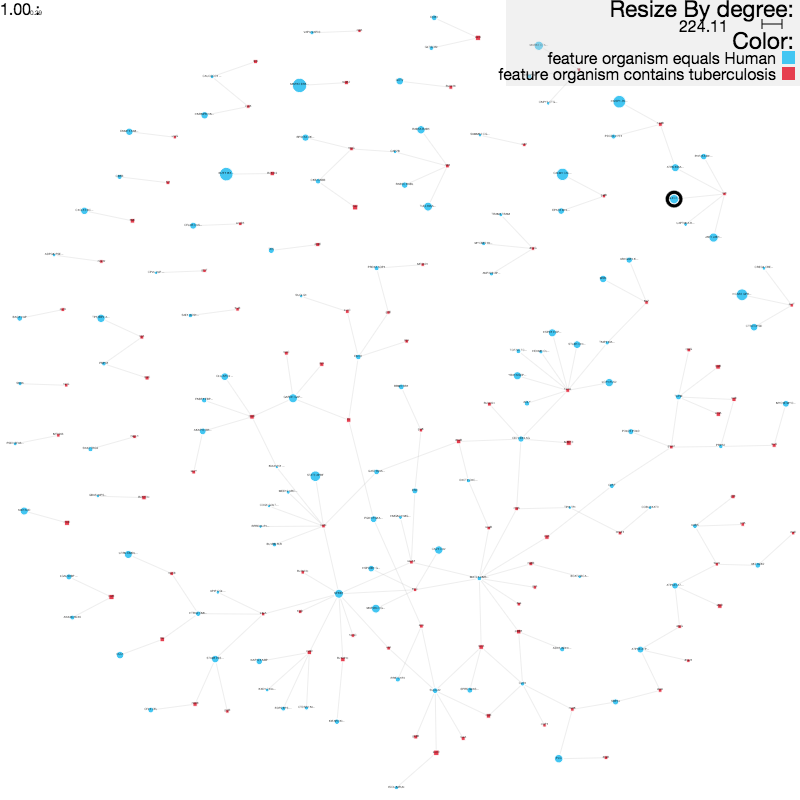
\includegraphics[width=5in]{figures/pinv_human_mtb.png}
\caption[Predicted functional interactions between MTB and Human]{Predicted functional interactions between MTB and Human. Blue circles are human proteins while red squares are from the MTB microorganism.
\label{fig:pinv_human_mtb}}
\end{figure}

\subsection{Research description}
This research is based on the fact that diseases such as tuberculosis are better understood from the relationships between the pathogenous and its host. Some of those relationships can be described as a protein protein interaction, where one protein belongs to the microorganism and the other to the host. Such interaction does not require to be direct (i.e proteins touching each other), and can be what is called a functional interaction, where for instance  the presence of one protein has an effect in the function of another protein. 

Although it is very relevant in the understanding of several biological processes, experimental studies of host-pathogen protein interactions are very scarce, and therefore computational prediction is the available alternative. In this study the authors used the interologs method in order to predict functional interactions between\emph{Mycobacterium tuberculosis} MTB and \emph{Homo Sapiens}. The predicted interactions were filtered, by selecting only the ones differently expressed during infection. The result set was then validated based in the known location of the proteins in the cell, verifying they belong to an area were cross-organism interaction is actually possible. 

The 190 proteins found were further analysed using functional and metabolical pathway knowledge, confirming the potential for some of those proteins to be drug target \cite{RAP2013}. These interactions also illustrate how MTB might acquire nutrients and how it modulates the host response to its advantage.

Figure \ref{fig:pinv_human_mtb} displays the interactions found in this work using PINV.


\subsection{Impact on PINV}

When the first results of this research were presented in a group meeting, the authors expressed the difficulties experienced while exploring the interaction datasets, especially when trying to generate visualisations that will help them to explain their findings. Given our experience with the visualisation projects described in section \ref{section:dasvisual} we took into the challenge of developing a tool that can support research projects that deal with this type of data on the web.

Periodical meetings with the authors of this research help us to define the requirements of PINV and methods to improve the user experience of researchers dealing with protein-protein interaction data. 

The first principle obtained from those meetings was that PINV needed to be more an exploration tool than a graphic generator or an analysis application. And from there comes the decision to have a repository that can be queried in order to extract only the information of interest, instead of loading the whole network in the visualiser, which ultimately ends up in the user requiring to preprocess the data in a separate tool.

\begin{figure}
\centering
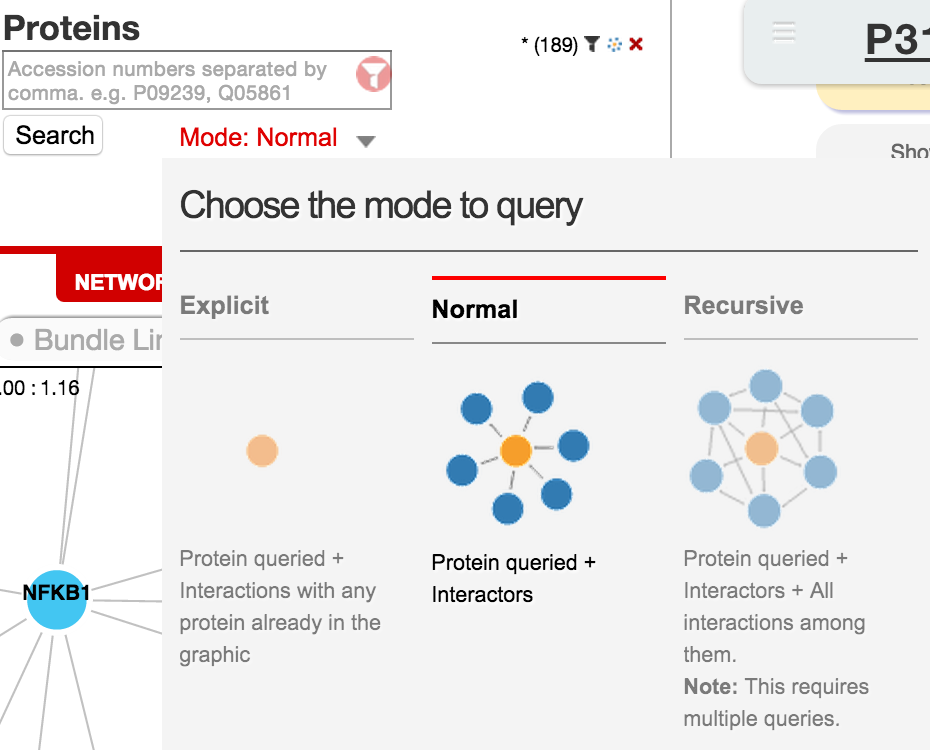
\includegraphics[width=4in]{figures/pinv_modes_query.png}
\caption[Three modes to query by ID in PINV]{Three modes to query by ID in PINV: Explicit, Normal and Recursive
\label{fig:pinv_modes_query}}
\end{figure}

It was with help of our collaborators that we defined the three modes to query by ID (Figure \ref{fig:pinv_modes_query}). PINV's firsts versions only included the normal mode in which a queried protein ID retrieves all the interactions were that protein ID has been reported, but later was pointed out that researchers some times prefer to limit their view to only a subset of proteins, and therefore we developed the explicit mode, and later on the recursive mode was also added as a combination.

Another learnings from these meetings were related to the data itself, on the one hand most of the interaction datasets have similarities, interaction data is  limited to the definition of pairs of biological molecules, information about the origin of the interaction is usually restricted to the method used to discover it. On the other hand, the protein data its heterogeneous, each project select different features to consider, for some, network intrinsic annotations (e.g. degree, closeness, etc.) are the features to consider, while for others, biological features are more relevant (e.g. functional class, cellular location, etc.). 

Based on this we defined that the upload of data to PINV requires two files, one defining the network with all the interactions between proteins and a second file with the annotations of interest for those proteins. A consequence of this open schema for protein data is that PINV widgets, have to adapt to the specificities of each dataset. For example the definition of rules to manipulate the graphic representation consider the features defined for each project, figure \ref{fig:pinv_human_mtb} for instance, uses the degree (i.e. number of connections in the network) of each protein to resize it. Thanks to that, it is easy to identify highly connected proteins, even when the current visualisation is filtering out most of the connections.

One more requirement gathered in this stage was to support direct manipulation of the visualisation; layouts are of great help to start analysing a network, however the researcher often requires to reorganise the network and manually locate some proteins in order to make more evident certain characteristics in the graphic. Therefore, proteins in PINV can be move by dragging them around the graphic, and the simulation forces can be stopped at any time.

\section{Orthologs in 3 Mycobactherium Organisms}\label{sec:orthologs}
\subsection{Research description}
This project presented a comparison between the functional networks of three related microorganisms: \emph{Mycobacterium tuberculosis} MTB, \emph{Mycobacterium leprae} MLP and \emph{Mycobacterium smegmatis}. Although sharing common ancestry, there are clear differences between them, some of which have been summarised in table \ref{tab:orthologs}.


\begin{table}[!ht]
        \begin{tabular}{|p{6cm}|p{3cm}|p{3cm}|p{3cm}|}
\hline 
\emph{feature} & \emph{MTB} & \emph{MLP} & \emph{MSM}\\
\hline 
Disease & Tuberculosis & Leprosy & \emph{non-pathogenic}\\
\hline 
Genome size & 4,411,532 & 3,268,203 & 6,988,209\\
\hline 
Number of proteins & 4136 & 1412 & 4853\\
\hline 
Doubling period (hours) & 24  & 500-670 & 3-4 \\
\hline 
        \end{tabular}
        \caption{Benchmarking between the main DAS servers.}
        \label{tab:orthologs}
\end{table}

The study identified the functional networks of the 3 organisms. The networks were created using STRING interactions as the base, but the network was enriched by including other 10 sources of functional interactions. One of them was a method designed as part of the project in order to be able to use co-expression analysis for MLP proteins, because the number of available experiments in this organism was limited to 4.

The final networks include only interaction which combined score range between medium or high confidence values, or ones with low values that are present in two or more sources. These networks were then analysed on a topological exclusive point of view, the found values and consideration about them can be seen in detail in \cite{AKI2013}.

The second part of the analysis compares the networks by pairs, in order to discover the biological consequences of the differences in the network. The strategy there was to select the most important proteins using network metrics (e.g. betweenness, degree and closeness) and proceed to compare them with their orthologs in the other networks. The comparison was done using among other features the functional class of the proteins. 

Sub-networks were then created with only the proteins that have orthologs in the other two organism, and similar comparisons are the ones explained above were done. Figure \ref{fig:pinv_orthologs} show an example of the type of analysis that can be done with the created networks. To start with, the authors have chosen one of the important proteins from MTB together with its orthologs in the other organisms, and by checking the neighbours of each protein and checking again for reported orthologs, it is easy to identified which interaction have been lost from one species to another.

\begin{figure}
\centering
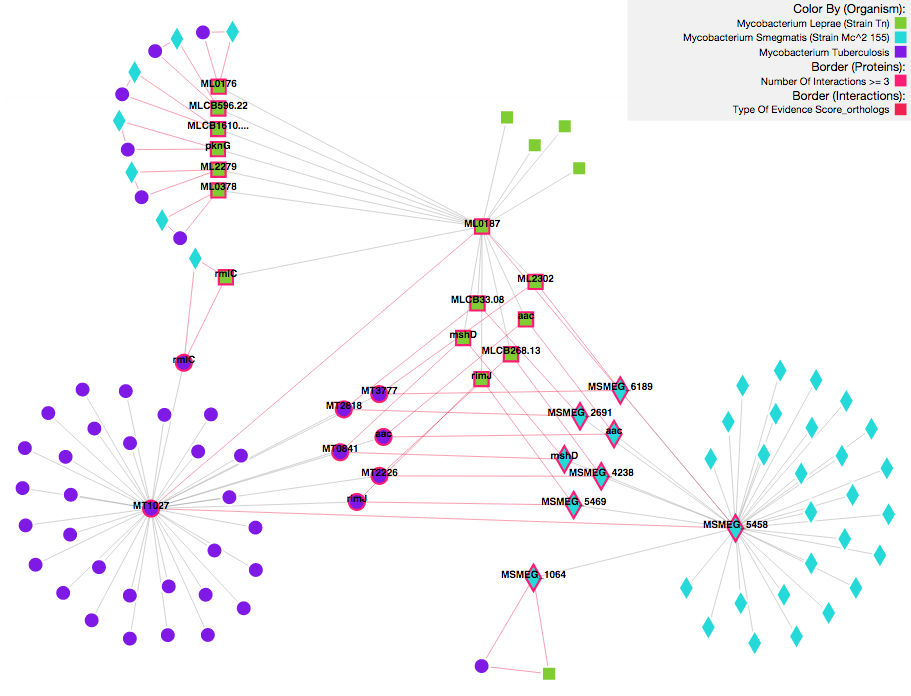
\includegraphics[width=\textwidth]{figures/pinv_orthologs.png}
\caption[Three orthologs proteins in MTB, MLP and MSM]{Three orthologs proteins in MTB, MLP and MSM: Q7D903, Q9CD64, A0R3F9. and their neighbours.
\label{fig:pinv_orthologs}}
\end{figure}

The interactive version of figure \ref{fig:pinv_orthologs} can be seen in \url{http://biosual.cbio.uct.ac.za/pinViewer.html?status=a512969c93f31b50926415e7fec14096.json}. This visualisation includes the different images used in the published article of this research \cite{AKI2013}, all of which were created using PINV.

\subsection{Impact on PINV}
This project was also held in the same research group where PINV was developed and the projects were executed simultaneously, which allow us to have again a first hand contact with the potential users of PINV while still in design stages. As a consequence some of the visualisation needs of this project influenced PINV development.

Firstly, this project required the display of 3 different species at the time, and makes evident that PINV should support the visualisation of interactions form multiple organisms. The implemented solution for PINV is to visualise the proteins in the network using different SVG symbols for each organism,  meaning that PINV will automatically choose one symbol from the available ones when protein of an organism not yet displayed is added. Currently there are 6 available symbols, but the list can be extended in future. Figure \ref{fig:pinv_orthologs} uses circles for MTB, squares for MLP and diamonds for MSM.

As a complement, we have extended the force-directed layout, including selective gravity forces, attracting each organism's proteins to different points in the graphic, this helps to automatically separate the proteins, and avoids cluttered areas of multiple species.

One particular characteristic in this project was the use of information of orthologs in between species, we decided to included it in the dataset to be uploaded to PINV as another type of interaction, creating an extra evidence score column in the data. This allows the user to reuse all the functionalities defined for interactions, for example, the spring forces in the network view work the same with this pseudo-interaction, and as a result the orthologs gets pull out of the main group interactions of each organism, in figure \ref{fig:pinv_orthologs} for instance, the proteins that share orthologs in the other organisms have been pulled to the centre of the graphic, so they are easily identifiable.

\begin{figure}
\centering
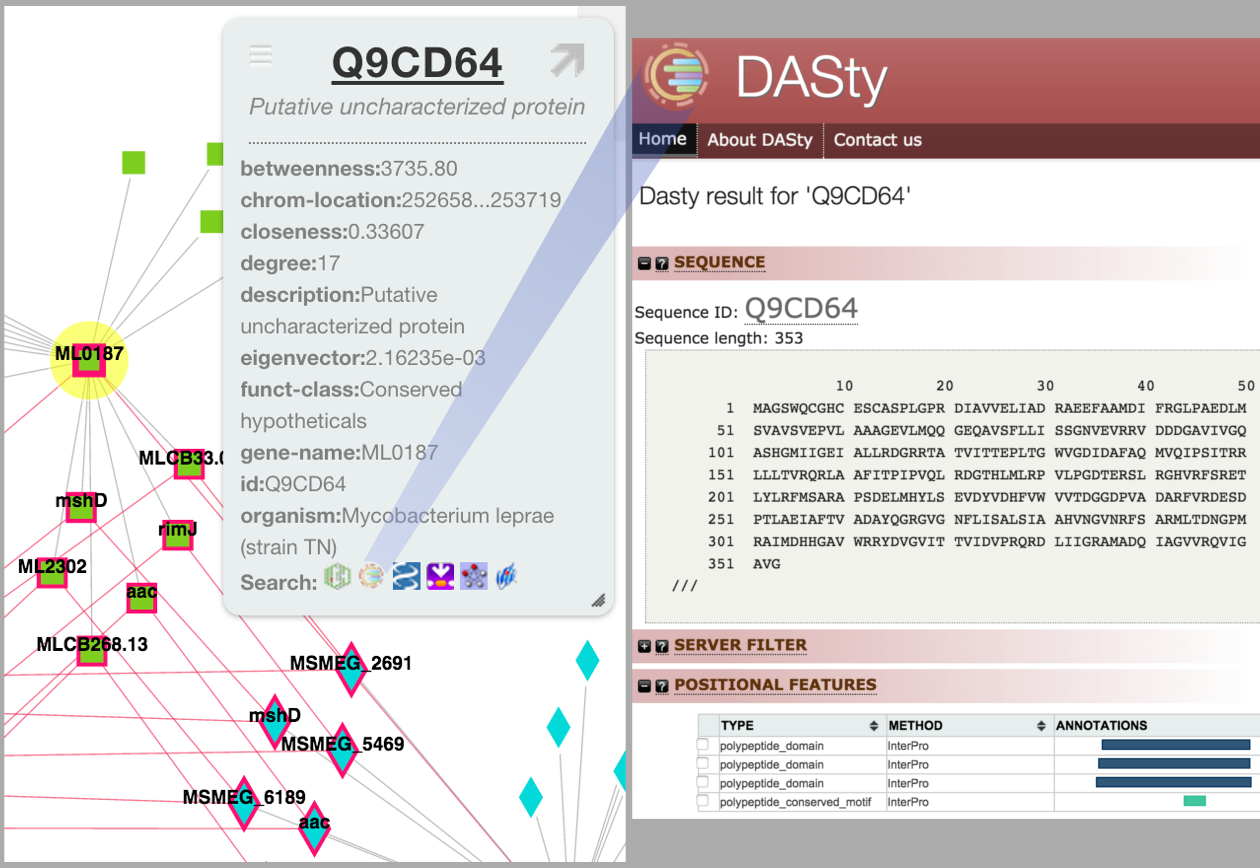
\includegraphics[width=5in]{figures/pinv2dasty.png}
\caption[Opening DASty3 from a protein of interest in PINV.]{Opening DASty3 from a protein of interest in PINV.
\label{fig:pinv2dasty}}
\end{figure}

Another requirement gathered during this collaboration was the need to open the exploration to other resources outside the PINV dataset, and been able to get access to more information from a protein of interest. Figure \ref{fig:pinv2dasty} shows in the left hand side the popup window that is displayed when a protein is selected in PINV, it includes the features that were upload in the dataset by the user. Moreover, PINV also shows links to several external resources at the bottom of the popup window, and for instance if the user clicks over the DASty3 logo another window will open this application searching for related information on the selected protein.



\section{Shotgun Analysis of Platelets From Dengue Patients}
\label{sec:dengue}
\subsection{Research description}
Real research example

"To generate a protein-protein interaction map and categorize the differential express proteins according biological processes classification on the Gene Ontology (GO) databank, we use the String 9.1 software and better vizualised by PINV. In a first interaction analysis, we input all the differentially express proteins and the proteins detected in only one condition, if in at least three replicates. Therefore, 344 proteins entries were listed; in with 253 were use, inasmuch as we exclude the protein isoforms indicated by a dash in the NextProt databank identifier. ???? proteins interactions were detected (Figure 2A). After generating the network, we performed a GO analysis with the interacting proteins, searching for relevant biological processes. Interesting, the eight most statically significant biological processes arising were related to “antigen processing and presentation” pathways and drew our attention in context of the dengue pathological state. This enriched pathways, whose the general GO identifier is GO:0019882 (p-value =  2.73E-10), were identified due to the presence of 19 differentially express proteins (ACTR1A, B*15, B-3501, ENSG00000229215, HLA-A, HLA-A*2410, HLA-ABC, HLA-B, HLA-B41, NPEPPS, PSMA6, PSMD13, PSMD4, RAB32, RAB35, RPS27A, UBA52, UBB and UBC). Some of these proteins are also related to proteasome/ubiquitinylation pathways (PSMA6, PSMD13, PSMD4, RPS27A, UBA52, UBB and UBC). Indeed, other important biological processes were highlight in this analysis: “protein polyubiquitination” (GO:0000209 with p-value = 5.88E-9 and 14 related proteins); “proteasomal protein catabolic process” (GO:0010498 with p-value = 4.69E-5 and 10 related proteins); and the already expected “platelet activation” (GO:0030168 with p-value = 8.36E-9 and 15 related proteins). To confirm whether these proteins directly interact with proteins related to the “platelet activation” pathway, a new interaction map was made focusing on these specific 41 non-redundant proteins involved in three ontologies (Figure 2B)." 

Figure \ref{fig:pinv_platelets_1}
Figure \ref{fig:pinv_platelets_2}

\subsection{Impact on PINV}
Filters and sharing

http://biosual.cbio.uct.ac.za/pinViewer.html?status=67049496bf99027c6d6f3ba33a9cb77b.json

\begin{figure}
\centering
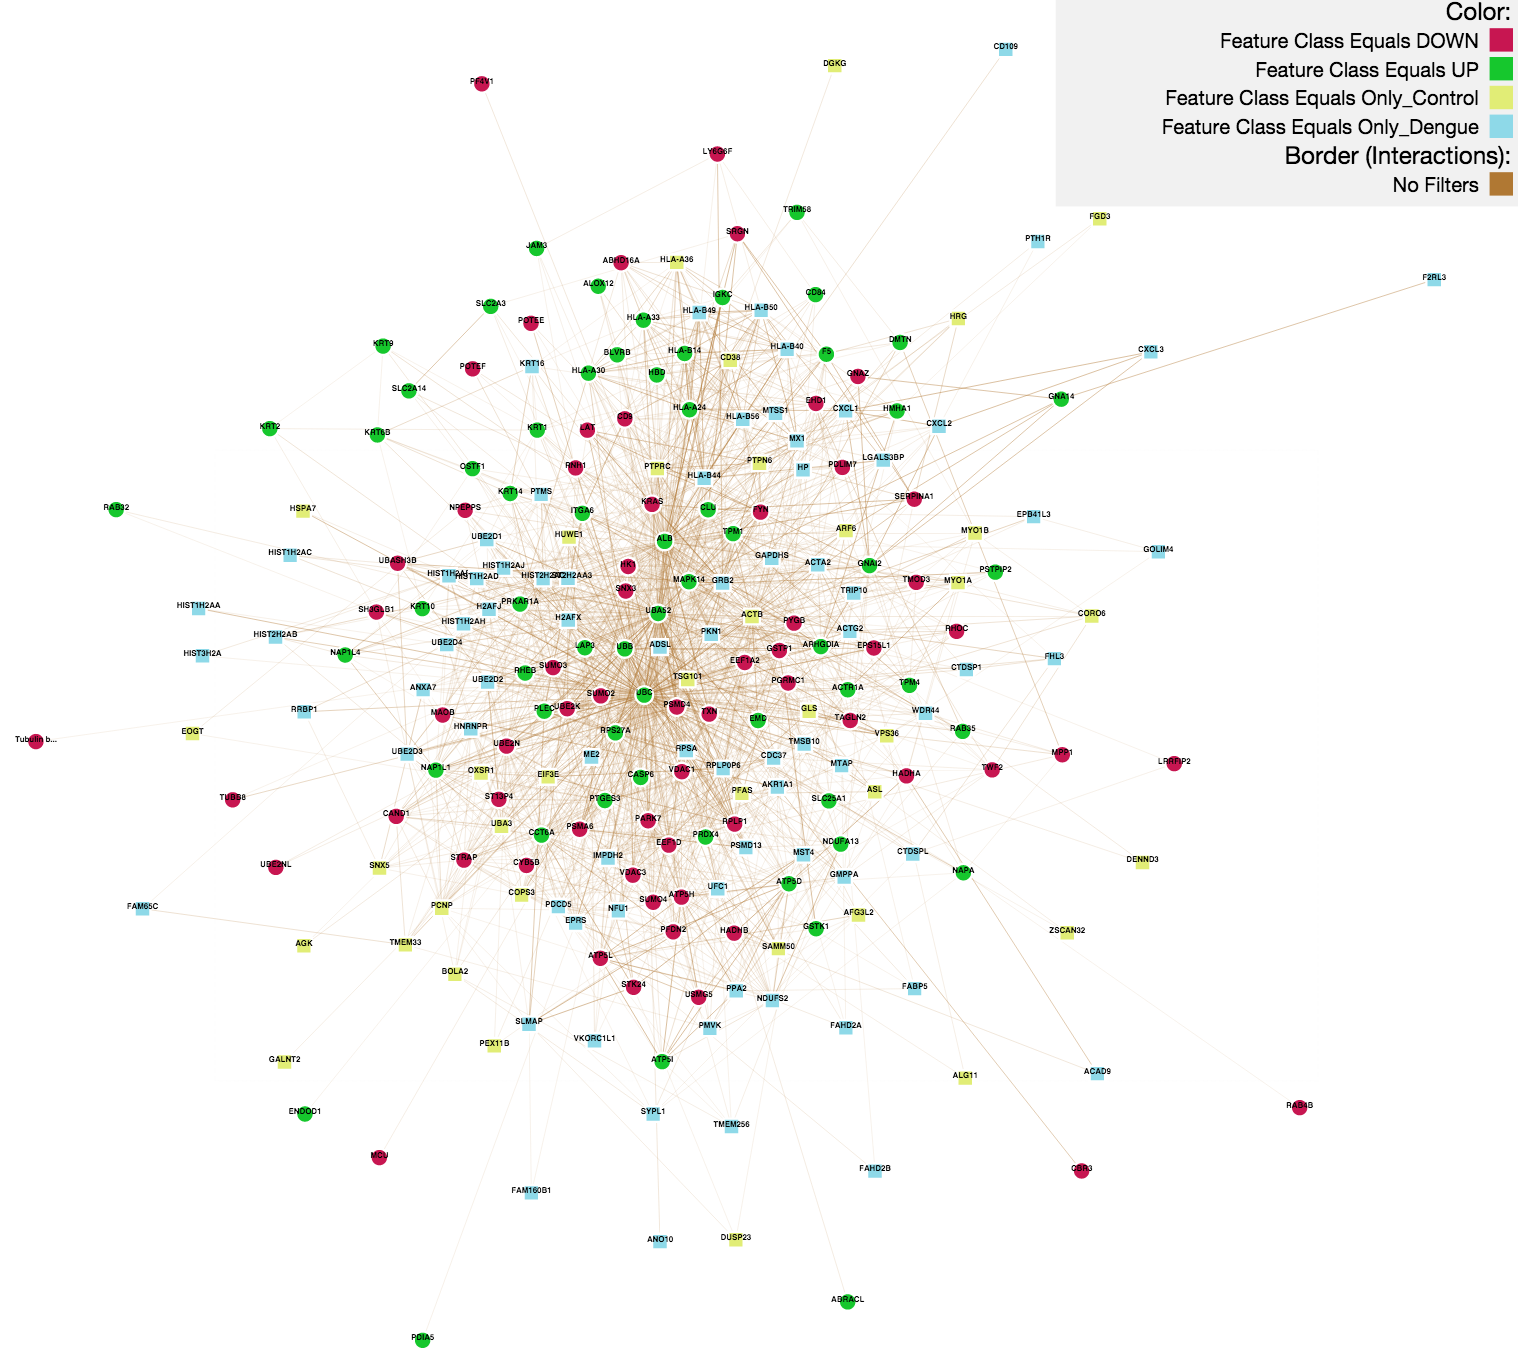
\includegraphics[width=5in]{figures/pinv_platelets_1.png}
\caption[Platelets1 ]{Platelets 1
\label{fig:pinv_platelets_1}}
\end{figure}

http://biosual.cbio.uct.ac.za/pinViewer.html?status=c1f68787907a83e27fab70be329582ce.json

\begin{figure}
\centering
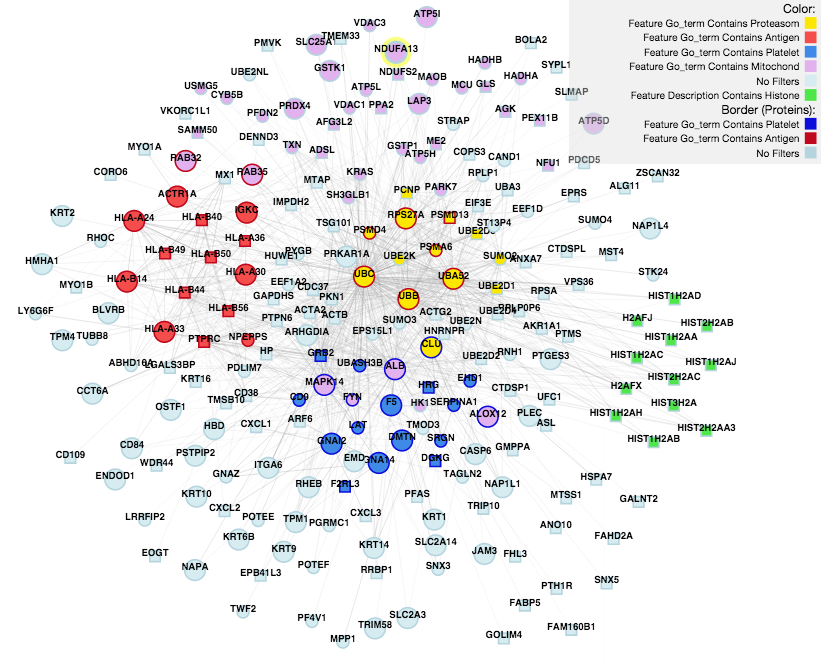
\includegraphics[width=\textwidth]{figures/pinv_platelets_2.png}
\caption[Platelets 2]{Platelets 2
\label{fig:pinv_platelets_2}}
\end{figure}

\section{Analysis of potential impact of SNPs on the human PPI network and gene expression}
\label{sec:pop_genetics}
\subsection{Research description}
This study investigates the impact of single nucleotide polymorphisms (SNP) on human particularly in the context of its protein-protein interaction network and taking into consideration gene expression in eight HapMap populations.

Previous studies have analysed consequences of SNPs in diseases, and some of them have included analysis to establish the relevance of the protein in which the mutation gets reflected in the human PPI network. Their finding suggests there are diseases that are caused by disrupted interactions. In \cite{HEE2014} the authors extend these studies in order to consider SNPs that are located in non-coding regions and the differences in allele frequencies between populations.

The project's methodology starts by integrating data from multiple resources of public domain: (i) human SNPs from NCBI (\url{ftp://ftp.ncbi.nlm.nih.gov/snp/organisms/human_9606_b141_GRCh37p13/VCF}), (ii) clinical related variations from NCBI (\url{http://www.ncbi.nlm.nih.gov/variation/docs/human_variation_vcf/#clinvar}) and Humsavar (\url{http://www.uniprot.org/docs/humsavar}), (ii) population data for allele frequencies (AF) and linkage disequilibrium (LD) for eight populations from HapMap (\url{ftp://ftp.ncbi.nlm.nih.gov/hapmap}), (iv) population gene expression data for the selected populations form Array Express (\url{http://www.ebi.ac.uk/arrayexpress/experiments/E-MTAB-264/}), (v) SNPs associated with gene expression levels reported in the publications \cite{STR2007}, \cite{LAP2013}, \cite{HAU2014} and \cite{WU2013}, and (vi) the Human PPI network compiled in the research described in the article \cite{RAP2013}.

Three centrality measurements were used to define the importance of each protein in the network: degree, betweenness and closeness. When analysing these values for proteins with non-synonymous SNP (nsSNP) in the human PPI network, the data showed that proteins containing nsSNPs have significantly lower centrality measures than proteins without nsSNPs. This is an indication that proteins with less interactions are less important for information flow, and therefore they can tolerate the amino acid change without having a major impact in the network.

A similar centrality analysis was executed with the subset of proteins that contain SNPs that have been identified as linked to diseases, and in this case it was shown that these proteins tended to have significant higher centrality measures than proteins without. Which can be explain by the implications on the structure change caused by the mutation, if it is considerable, it might inhibit some of the stablished interactions. This might not be critical in proteins with an small number of interactions, but in central proteins the effect can collapse the network, and hence the disease.

The integrated dataset can be used to explore particular diseases and potentially improve understanding of inter-population variation. An example of it was included in the research, in which proteins with SNPs related to hypertension were selected: ADD1, NOS3, AGT and KCNMB1. Figure \ref{fig:pinv_human_snps} shows the subnetwork of these proteins only displaying high confidence interactions (score ≥ 0.7) in which both of the proteins contained a nsSNP and at least one of the proteins contained a clinSNP associated with hypertension. The figure is colour coded to highlight the significant differences in AF and gene expression between African populations. 

\begin{figure}
\centering
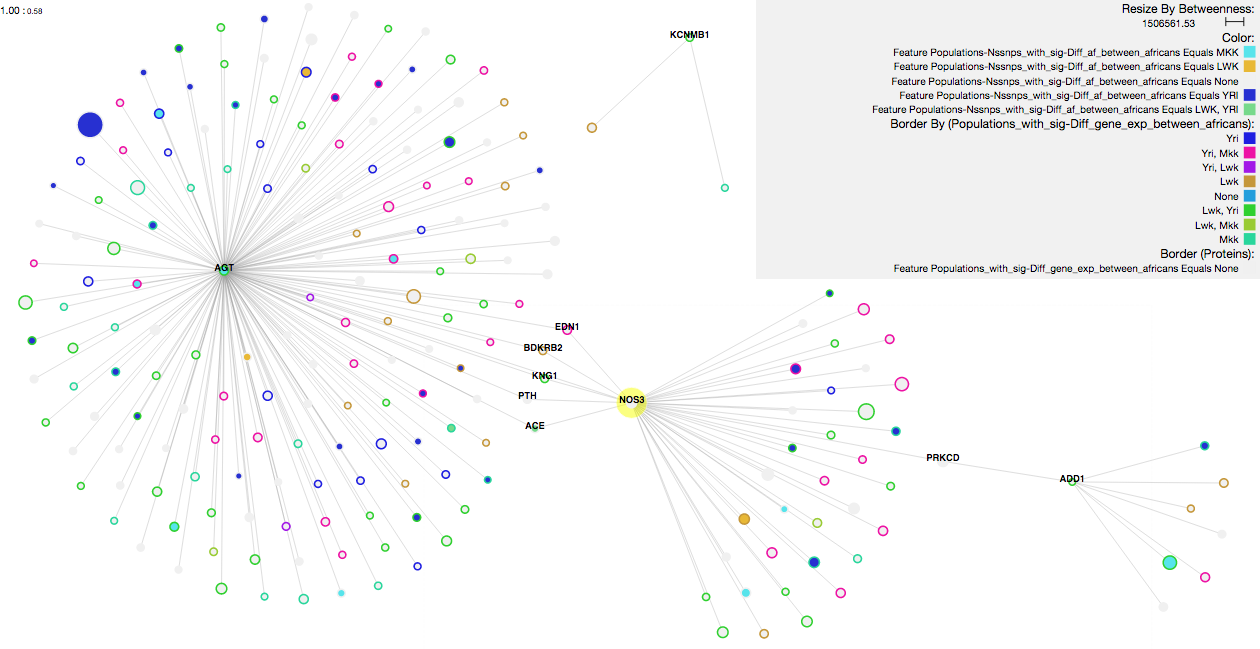
\includegraphics[width=\textwidth]{figures/pinv_human_snps.png}
\caption[Interactions between proteins with a hypertension clinSNP]{Interactions between proteins with a hypertension clinSNP and proteins with nsSNPs in the context of AF and gene expression differences between African populations.
\label{fig:pinv_human_snps}}
\end{figure}

Similar comparison graphics are included in \cite{HEE2014} among other populations and the implications of the identified proteins is discussed there in more detail. All the graphics were created using PINV. An interactive version of Figure \ref{fig:pinv_human_snps} is available in \url{http://biosual.cbio.uct.ac.za/pinViewer.html?status=dc029e8ef629cd4fed0c4a1509a70ef7.json}

\subsection{Impact on PINV}
The case explained above where hypertension related proteins were analysed on the context of PPI networks was completely carried on using PINV. The dataset of this research was uploaded to the PINV server and is available under this URL: \url{http://biosual.cbio.uct.ac.za/pinViewer.html?core=HumanHapMapSNPs}. 

The authors were able to explore their data by defining different combinations of filters, for example, figure \ref{fig:pinv_prefilters_snp} is a snapshot of the selected filters used for the generation of figure \ref{fig:pinv_human_snps}, which we will describe from top to bottom: 
\begin{enumerate}
\setlength\itemsep{-0.5em}
\item This filters the whole human PPI network (1298519 interactions) in order to only include the ones with high confidence interactions (score ≥ 0.7) a total of 306453 interactions.
\item The second filter helps the researchers to focus only in the interactions between proteins with nsSNP. There are 182755 interactions in the whole network complying with this restriction, and in combination with the first filter, the subset gets reduced to 50211 interactions.
\item There is a total of 209540 interactions where at least one of the proteins has a SNP which has been linked to a disease, and from that 9662 interactions also pass the previous filters.
\item It select all the interactions where at least one of the proteins contains the term ``\emph{hypertension}'' on a field were all the diseases related with SNPs present in a protein are listed. 1711 interactions were found this way, and the intersection with the other filters produces 212 interactions.
\end{enumerate}
\begin{figure}
\centering
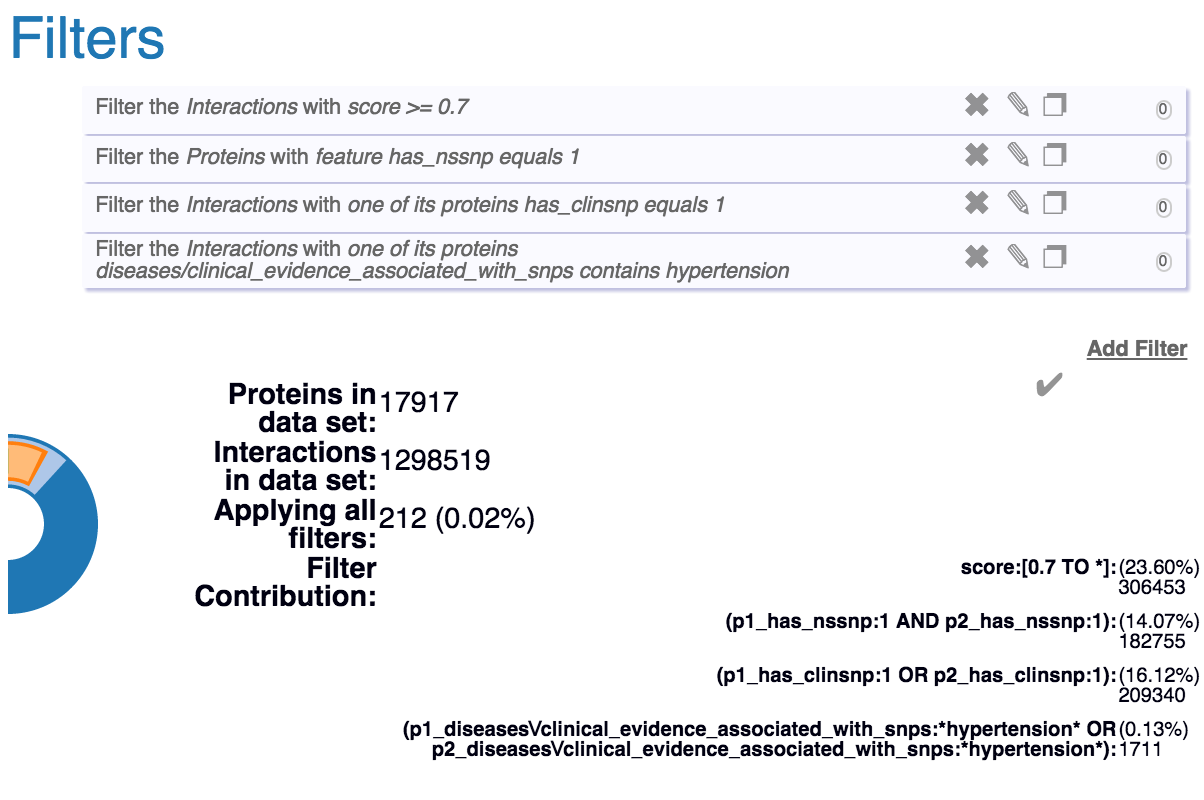
\includegraphics[width=5in]{figures/pinv_prefilters_snp.png}
\caption[Selection of filters for image \ref{fig:pinv_human_snps}]{Selection of filters for image \ref{fig:pinv_human_snps}
\label{fig:pinv_prefilters_snp}}
\end{figure}

From the result graphic only 4 proteins have been directly identified to be related with hypertension, and although it wasn't  imposed by the filters, the result subnetwork connects 3 of the proteins with one degree of separation in between them. Which is an indication of agreement with the original assumption of the research: some diseases can be better understood by studying their related proteins in context of the human PPI network.

Once the network is identified, other factors can be analysed, for instance the colour coding in figure \ref{fig:pinv_human_snps} identifies differently expressed proteins in different african populations. This can help to understand why a disease affects populations in different ways. It is now part of our future plan to define a strategy to compare networks that share the same structure, and for example been able to see in the same graphic a comparison between the analysis for african populations \emph{v.s.} european or american populations. 

The example presented in this research demonstrates how PINV can be used for the exploration of PPI data, and how the use of filters supplies an alternative to navigate the data when the accession numbers of the proteins of interest are still to be found. A similar protocol to the described above can be use to explore other clinical conditions, for instance one of the appendices of \cite{HEE2014} is a similar visualisation but for cancer related proteins. This is an example of a dataset that by being public in PINV can benefit more than one research.

While the project was being executed, the authors gave us constant feedback and many suggestions to improve PINV. For instance, several issues were corrected in the uploading process because of the large number of interactions that needed to be upload.

%to show the clustering in action!! 


